%% ----------------------------------------------------------------
%% Thesis.tex -- main
%% ---------------------------------------------------------------- 

\documentclass[a4paper, 10pt, oneside]{memoir}
%% Use the option citeauthor to be able to use citet. The default cite will still work.
\usepackage[citeauthor]{basilea}

%% ----------------------------------------------------------------

\title				{Optimizing Symbolic Execution Through Taint Analysis and Path Prioritization}
\thesistype			{Bachelor thesis}

\department 		{Department of Mathematics and Computer Science}
\faculty			{Natural Science Faculty of the University of Basel}
\research		    {Databases and Information Systems (DBIS) Group \\ \url{https://dbis.dmi.unibas.ch/}}

\examiner    		{Dr. Marco Vogt}
\supervisor  		{Prof. Dr. Christopher Scherb}

\authors     		{Ruben Hutter}
\email				{ruben.hutter@unibas.ch}
\immatriculnr		{2020-065-934}

\date				{02.07.2025}

% switch here for the german logo to logo-de
\ulogo				{Template/logo-en} 


%% ----------------------------------------------------------------
\begin{document}

% for english use \selectlanguage{english}, for german use \selectlanguage{ngerman}
\selectlanguage{english}

\thesisfront
\maketitle
\pagestyle{thesis}
%% ----------------------------------------------------------------
% % !TEX root = ../Thesis.tex
\chapter{Acknowledgments}

I would like to express my sincere gratitude to Prof. Dr. Christopher Scherb for his supervision and guidance throughout this thesis. His expertise in program analysis and symbolic execution provided essential direction for this research.

I am grateful to Dr. Marco Vogt for his role as examiner and for facilitating the opportunity to pursue this research topic. His feedback and suggestions helped refine both the technical approach and the presentation of this thesis.

I would like to thank Ivan Giangreco for providing the LaTeX thesis template used for this document, which greatly facilitated its formatting and structure.

I also acknowledge my fellow student Nico Bachmann for developing the Schnauzer visualization library, which enhanced the presentation and analysis of the results.

I thank my family and friends for their encouragement and support during my studies, which made completing this thesis possible.

Finally, I acknowledge the developers of the angr binary analysis framework, whose comprehensive platform enabled the implementation of the techniques described herein.

%% ----------------------------------------------------------------
% !TEX root = ../Thesis.tex
\chapter{Abstract}

Symbolic execution is a powerful program analysis technique widely used for vulnerability discovery and test case generation. However, its practical application is often hampered by scalability issues, primarily due to the "path explosion problem" where the number of possible execution paths grows exponentially with program complexity. This thesis addresses this fundamental challenge by proposing an optimized approach to symbolic execution that integrates taint analysis and path prioritization.

The core contribution is a novel exploration strategy that moves away from uniform path exploration towards targeted analysis of security-critical program behaviors. The approach prioritizes execution paths originating from memory allocations and user input processing points, as these represent common sources of vulnerabilities. By leveraging dynamic taint analysis, the system identifies and tracks data flow from these critical sources, enabling the symbolic execution engine to focus computational resources on paths influenced by tainted data while deprioritizing paths with no dependency on external inputs.

% TODO: Benchmark to test if this is actually true
The implementation integrates this taint-guided exploration strategy with the angr symbolic execution framework, introducing a scoring mechanism that dynamically adjusts path prioritization based on taint propagation. The effectiveness of this optimization is evaluated through comparative analysis, examining runtime efficiency, path coverage quality, and vulnerability discovery capabilities. Results demonstrate that this approach can significantly reduce the search space while maintaining or improving the detection of security-relevant program behaviors, making symbolic execution more practical for large and complex software systems.

%% ----------------------------------------------------------------
\thesistoc
%% ----------------------------------------------------------------
%\thesisnomencl
%% ----------------------------------------------------------------
\thesismain
% !TEX root = ../Thesis.tex
\chapter{Introduction}

This is the introduction to the thesis template. The goal is to give students a starting point on how to format and style their Bachelor or Master thesis\footnote{This document also shows how to use the template.}. 

Please make sure to always use the most current version of this template, by downloading it always from the original git repository:
\begin{center}
	\url{http://www.github.com/ivangiangreco/unibas-latex} 
\end{center}

We will use throughout this tutorial some references to Turing's imitation game~\cite{turing:1950} and the Turing machine~\cite{turing:1936}. You may be interested in reading these papers.

\vspace{1em}
The package comes with an option regarding the bibliography style.
You can include the package with
\begin{verbatim}
\usepackage[citeauthor]{basilea}
\end{verbatim}
to be able to cite authors directly with
\begin{verbatim}
\citet{turing:1950}
\end{verbatim}

If the option is enabled, then the following reference should print Turing [2]:~\citet{turing:1950}


% !TEX root = ../Thesis.tex
\chapter{Body of the Thesis}

This is the body of the thesis.

\section{Structure}
\label{sec:my-label}

\subsection{Sub-Section}

\subsubsection{Sub-Sub-Section}

\paragraph{Paragraph}

\subparagraph{Even Sub-Paragraph}

This is the body text. Make sure that when you reference anything you use labels and references. When you refer to anything, you normally capitalise the type of object you reference to, e.g. Section~\ref{sec:my-label} instead of section~\ref{sec:my-label}. You may also just use the \texttt{cref} command and it will generate the label, e.g., for \cref{sec:my-label}, we did not specify the word ``Section''.

Hint: Try to structure your labels as it is done with \texttt{sec:my-label} and \texttt{fig:machine}, etc.



\section{Equations}
A Turing Machine is a 7-Tuple:
\begin{equation}
    M = \langle Q, \Gamma, b, \Sigma, \delta, q_0, F \rangle
\end{equation}
A Turing Machine is a 7-Tuple even if defined in the text, as in $M = \langle Q, \Gamma, b, \Sigma, \delta, q_0, F \rangle$.




\section{Tables}
Some tables can also be used as shown in \cref{tab:table}\footnote{Table captions are normally above the table.}. Remember that tables might be positioned elsewhere in the document. You can force positioning by putting a \texttt{ht!} in the definition.

\begin{table}[ht!]
\centering
\caption{Frequency of Paper Citations. By the way: Make sure to put the label always after the caption, otherwise \LaTeX{} might reference wrongly!}
\begin{tabular}{lcl} \toprule
Title&$f$&Comments\\ \midrule
The chemical basis of morphogenesis & 7327 & \\ 
On computable numbers, with an application to the ... & 6347 & Turing Machine\\
Computing machinery and intelligence & 6130 & \\ \bottomrule
\end{tabular}
\label{tab:table}
\end{table}




\section{Figures}
Figures are nice to show concepts visually. For organising well your thesis, put all figures in the Figures folder. Figure~\ref{fig:machine} shows how to insert an image into your document. \Cref{fig:tm} references a figure with multiple sub-figures, whereas the sub-figures are referenced by \cref{fig:tm:tm1}, etc. \todoMissing{Description of figure.}

\begin{figure}
\centering
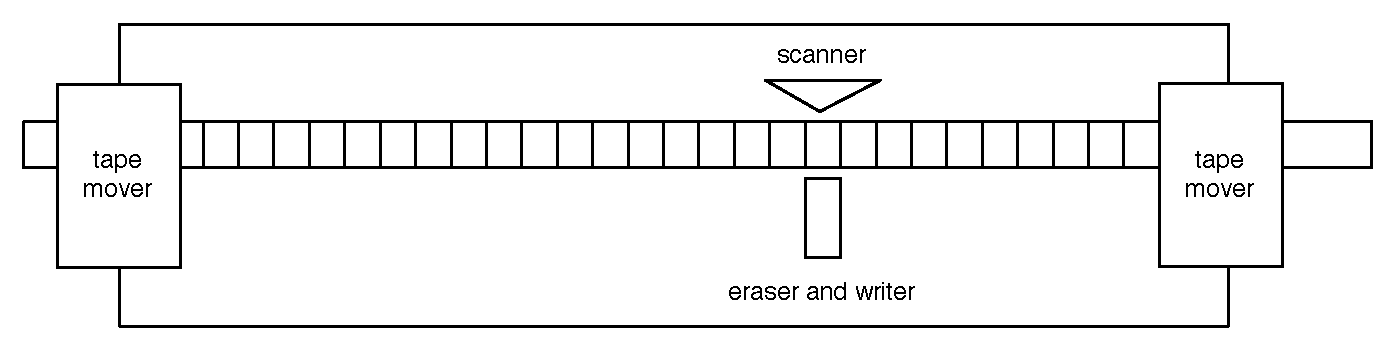
\includegraphics[width=0.9\textwidth]{turingmachine}
\caption{A Turing machine.}
\label{fig:machine}
\end{figure}


\begin{figure}
\centering
\subbottom[Turing Machine 1\label{fig:tm:tm1}]{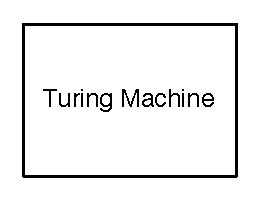
\includegraphics[width=0.2\textwidth]{block}}
\subbottom[Turing Machine 2\label{fig:tm:tm2}]{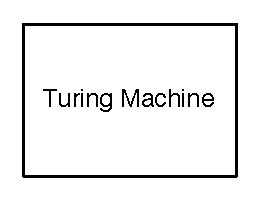
\includegraphics[width=0.2\textwidth]{block}}
\subbottom[Turing Machine 3\label{fig:tm:tm3}]{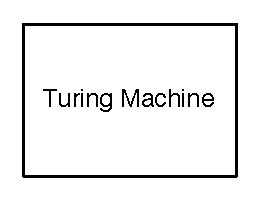
\includegraphics[width=0.2\textwidth]{block}}
\subbottom[Turing Machine 4\label{fig:tm:tm4}]{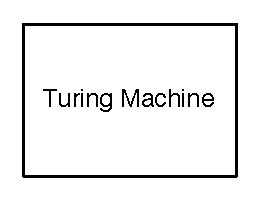
\includegraphics[width=0.2\textwidth]{block}}
\caption{Plots of four Turing machines}
\label{fig:tm}
\end{figure}




\section{Packages}
These packages might be helpful for writing your thesis:

\begin{description}
	\item[\texttt{caption}] to adjust the look of your captions
	\item[\texttt{glossaries}] for creating glossaries (also list of symbols)
	\item[\texttt{makeidx}] for indexes and the back of your document
	\item[\texttt{algorithm, algorithmicx, algpseudocode}] for adding algorithms to your document
\end{description}
% !TEX root = ../Thesis.tex
\chapter{Conclusion}
This is a short conclusion on the thesis template documentation. If you have any comments or suggestions for improving the template, if you find any bugs or problems, please contact me. 

\vspace{2cm}

Good luck with your thesis!
%\input{./Chapters/Chapter4}
%\input{./Chapters/Chapter5}
%\input{./Chapters/Chapter6}
%\input{./Chapters/Chapter7}
%% ----------------------------------------------------------------
\thesisappendix
\thesisbib
\begin{appendices}
	% !TEX root = ../Thesis.tex
\chapter{Appendix}

\section{State Explosion Test Program Source Code}

\begin{lstlisting}[language=C, label={lst:state_explosion_test_program}]
#include <stdio.h>
#include <string.h>

void create_many_string_states(char *input) {
    // Create branching based on string content (tainted)
    if (strlen(input) > 10) {
        printf("Long input\n");
    } else {
        printf("Short input\n");
    }

    if (input[0] == 'A') {
        printf("Starts with A\n");
    } else if (input[0] == 'B') {
        printf("Starts with B\n");
    } else {
        printf("Starts with other\n");
    }
}

void untainted_integer_branching() {
    int static_val = 25;  // Hardcoded, not tainted

    // Classical angr will explore these, TraceGuard should skip
    if (static_val > 20) {
        printf("Static val > 20\n");
    }
    if (static_val % 5 == 0) {
        printf("Static val divisible by 5\n");
    }
    if (static_val < 30) {
        printf("Static val < 30\n");
    }
}

void critical_vulnerability(char *dangerous_input) {
    char tiny_buffer[6];  // Extremely small
    strcpy(tiny_buffer, dangerous_input);  // Obvious overflow
    printf("Critical: %s\n", tiny_buffer);
}

int main() {
    char user_input[400];

    // Untainted branching - TraceGuard should skip
    untainted_integer_branching();

    printf("Enter string input: ");
    if (fgets(user_input, sizeof(user_input), stdin)) {
        // Remove newline
        user_input[strcspn(user_input, "\n")] = 0;

        // This creates tainted string-based branching
        create_many_string_states(user_input);

        // Clear vulnerability with tainted data
        critical_vulnerability(user_input);
    }
    return 0;
}
\end{lstlisting}
 
\end{appendices}
%% ----------------------------------------------------------------
\thesisback
\iflanguage{english}
  {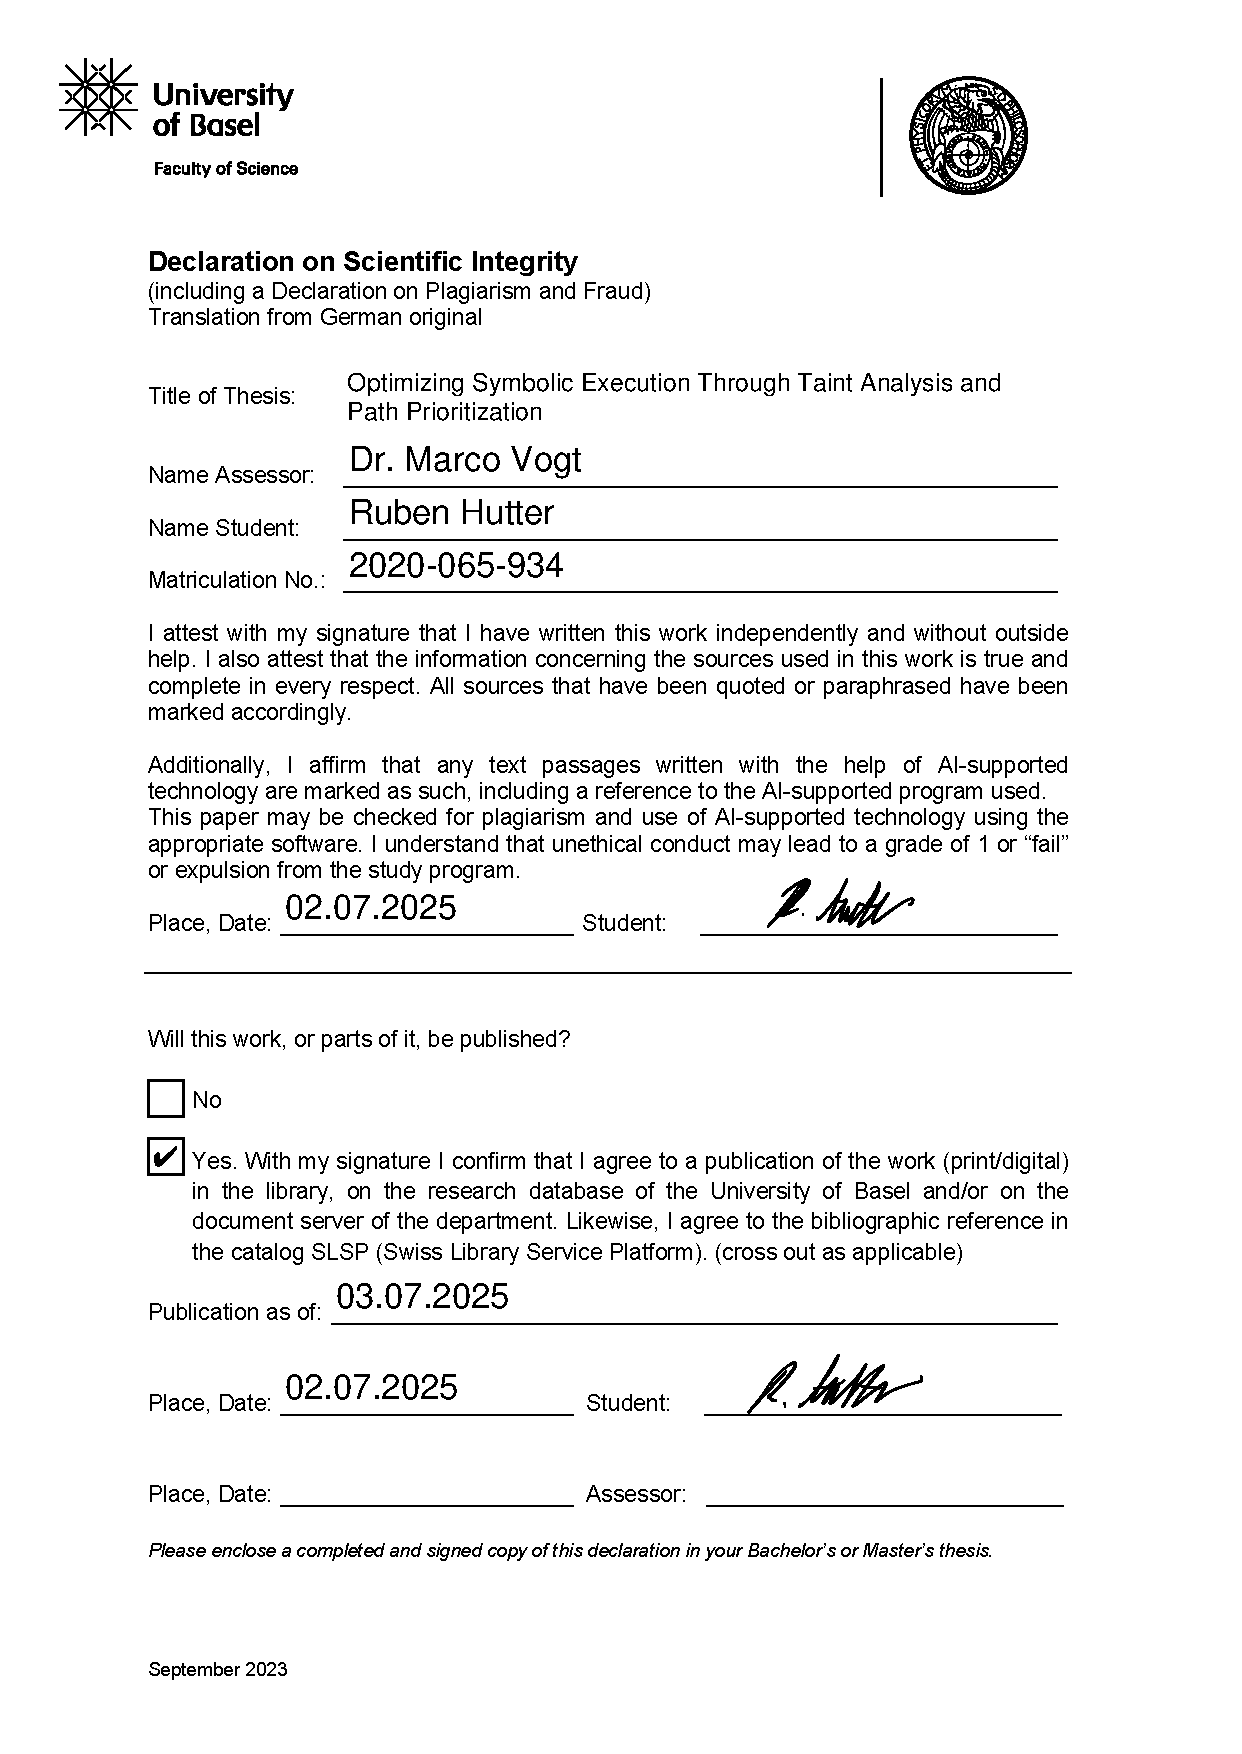
\includepdf{./Back/wissensch_Redlichkeit_E_09-2023.pdf}}
  {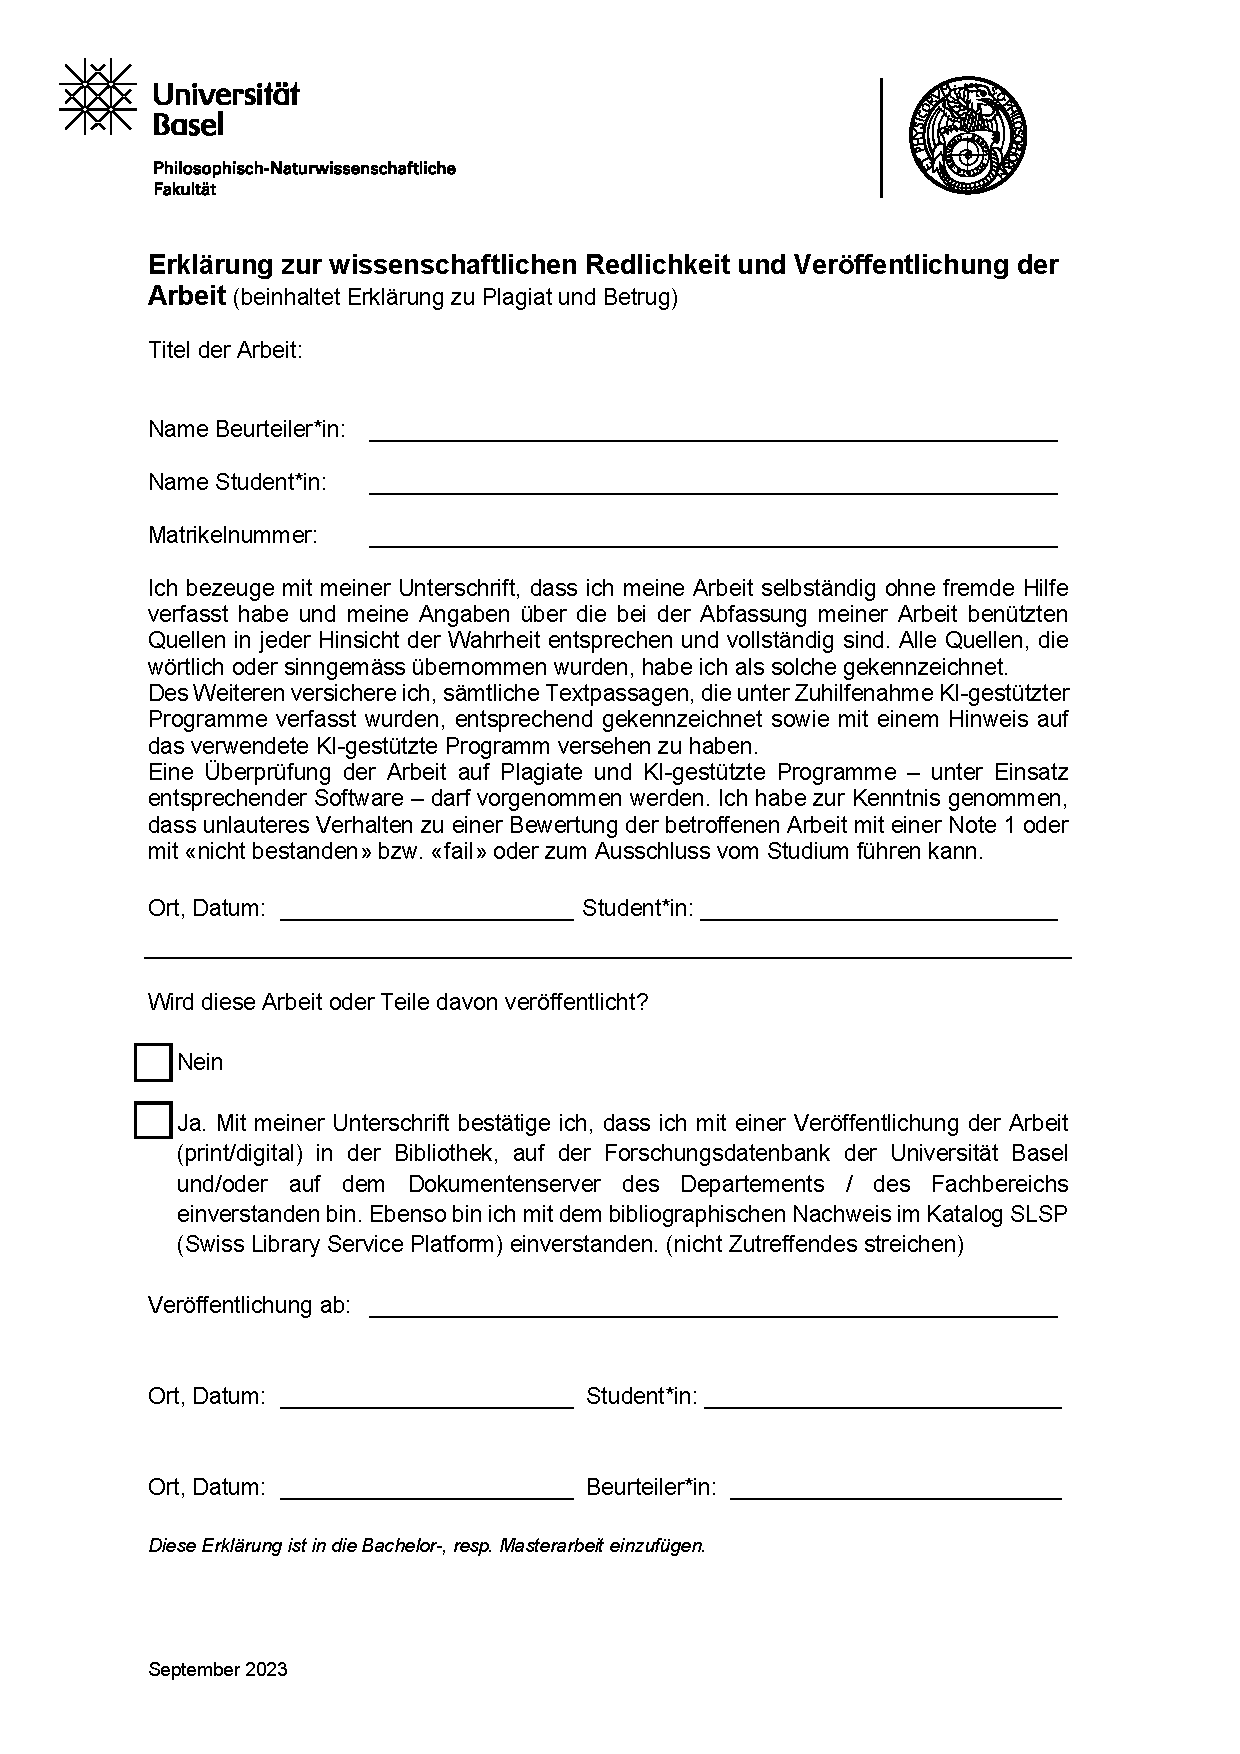
\includepdf{./Back/wissensch_Redlichkeit_D_09-2023.pdf}}
%% ----------------------------------------------------------------
\end{document}
%% ----------------------------------------------------------------
